\documentclass[10pt]{exam}
\usepackage[icp]{template-for-exam}
\usepackage{multicol}
\usepackage{pgfplots}
\pgfplotsset{
  compat=1.18, 
  every axis/.append style={
    grid=major,
    xtick={0,1,...,25},
    ytick={-10,-9,...,15},
    grid style = dashed,
  },
  empgraph/.append style={
    xmin=0, xmax=9,
    ymin=0, ymax=6,
    width  = 5cm,
    height = 4cm,
    ylabel = {position},
    xlabel={time},
    xtick = \empty,
    ytick = \empty,
    axis y line = left,
    axis x line = bottom,
  },
  soln/.append style={
    red,
    domain=0:7
  }
}
%\printanswers
\shadedsolutions

\title{Unit P1 Review (Motion)}
\author{Rohrbach}
\date{\today}

\begin{document}
\maketitle

\begin{questions}

  \question
    Define the following terms in your own words. 
    \begin{parts}
        \part Velocity:
          %
          \begin{solution}[\stretch{1}]
            how fast an object is moving and its direction (measured in m/s)
          \end{solution}

        \part Acceleration:
          %
          \begin{solution}[\stretch{1}]
            the rate that velocity changes (measured in m/s/s or \SI{}{\meter\per\second^2})
          \end{solution}
    \end{parts}

  \question
    What is the acceleration of a car moving at a constant speed in a straight line?  How do you know?
    %
    \begin{solution}[\stretch{1}]
      zero.  The velocity is not changing.
    \end{solution}

  \question
    What are the three ways to accelerate?
    %
    \begin{solution}[\stretch{1}]
      speed up, slow down, change direction
    \end{solution}

    \question
    Draw the following distance-time graphs.

    \newcommand{\empgraph}[1]{
      \par
      \begin{tikzpicture}
        \begin{axis}[empgraph]
        \ifprintanswers
          \addplot[soln] {#1};
        \fi
        \end{axis}
      \end{tikzpicture}
    }

    \begin{multicols}{2}
      \begin{parts}
        \part Not moving \empgraph{3}
        \part Forward at a constant speed \empgraph{0.6*x}
        \part Backward at a constant speed \empgraph{5-0.6*x}
        \part Forward and speeding up \empgraph{(x/3)^2}
        \part Backward and speeding up \empgraph{-(x/3)^2+5}
        \part Forward and slowing down \empgraph{-(x/3-2.1)^2+5}
      \end{parts}
    \end{multicols}

  \pagebreak
  
  \question
    The motion of an object during a 16 second time period is graphed below. 

    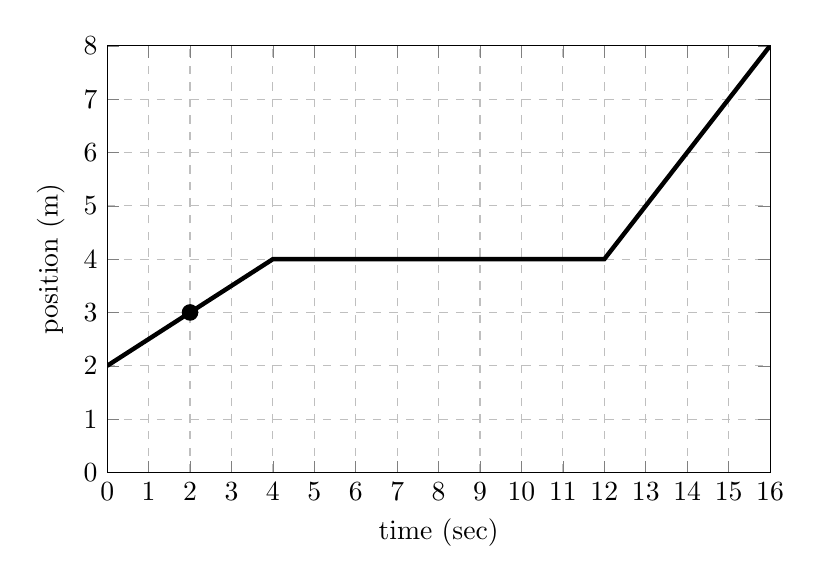
\begin{tikzpicture}
      \begin{axis}[
          xmin=0, xmax=16,
          ymin=0, ymax=8,
          width  = 10cm,
          height = 7cm,
          ylabel = {position (m)},
          xlabel={time (sec)},
      ]
        \addplot [ultra thick] table {
          x   y
          0   2
          4   4
          12  4
          16  8
        };
        \fill (2,3) circle (3pt);
      \end{axis}
    \end{tikzpicture}

    \begin{parts}
        \part 
          What is the object's position at 2 seconds?
          %
          \begin{solution}[\stretch{1}]
            3 meters
          \end{solution}
        
        \part
          How far has the object traveled from the beginning of the motion ($t=\SI{0}{\second}$) to the point indicated by the dot on the graph ($t=\SI{2}{\second}$)?
          %
          \begin{solution}[\stretch{1}]
            1 meter
          \end{solution}
        
        \part
          What is the object doing at 2 seconds? (for example, moving forward and speeding up, moving backward at a constant speed, standing still, etc.)
          %
          \begin{solution}[\stretch{1}]
            moving forward at a constant speed
          \end{solution}
        
        \part
          What distance did the object between when it started ($t=\SI{0}{\second}$) and ended ($t=\SI{16}{\second}$) its motion.
          %
          \begin{solution}[\stretch{1}]
            6 meters
          \end{solution}

        \part
          What is the velocity of the object between 0 seconds and 4 seconds?
          %
          \begin{solution}[\stretch{1}]
            0.5 m/s
          \end{solution}

        \part
          What is the velocity of the object between 12 seconds and 16 seconds?
          %
          \begin{solution}[\stretch{1}]
            1 m/s
          \end{solution}

    \end{parts}
  
  \question
    A position versus time graph of a car is shown below. Explain in at least two sentences what the car is doing.  
  
    \begin{tikzpicture}
        \begin{axis}[
            xmin=0, xmax=9,
            ymin=0, ymax=6,
            width  = 8cm,
            height = 5cm,
            ylabel = {position},
            xlabel={time},
            xtick = \empty,
            ytick = \empty,
            axis y line = left,
            axis x line = bottom,
        ]
          \addplot [ultra thick] table {
            x   y
            0.5 5
            4   5
            8   0.5
          };
        \end{axis}
        \ifprintanswers
          \node[fill=SolutionColor] at (9,2) {The car is not moving and then moves backwards at a constant speed};
        \fi
      \end{tikzpicture}

  \pagebreak
  
  \question
    Draw a graph for the following situation:
    \begin{parts}
      \part
        I start at school and drive forward 2 miles in 4 minutes.  
      \part
        Then I get stopped at a red light for 1 minute.  
      \part 
        The light turns green and I go forward 2 miles in 5 minutes.
      \part 
        I turn around and go back to school because I forgot my phone.  It makes me 6 minutes to get back.
      \part 
        It then takes me 4 minutes to go 1 mile forward because of traffic.
    \end{parts}

    \begin{tikzpicture}
      \begin{axis}[
          xmin=0, xmax=20,
          ymin=0, ymax=5,
          width  = 15cm,
          height = 7cm,
          ylabel = {position (miles)},
          xlabel={time (minutes)},
      ]
      \ifprintanswers
        \addplot[soln] table {
          x   y
          0   0
          4   2
          5   2
          10  4
          16  0
          20  1
        };
      \fi
      \end{axis}
    \end{tikzpicture}

  \newcommand{\ansblank}{
    \ifprintanswers
    \else
      \ku
    \fi
    \vs
  }

  \question
    How much time does it take for a car to travel at 28.4 m/s to travel 3000 meters? 
    %
    \begin{solution}
      \begin{align*}
        v &= \SI{28.4}{\meter\per\second} 
                            & v &= \frac{d}{t} \\
        d &= \SI{3000}{\meter}
                            & 28.4 &= \frac{3000}{t} &
                              t &= \SI{105.63}{\second}
      \end{align*}
    \end{solution}
    \ansblank

  
  \question
    If a car is initially traveling forward at 15 m/s, how fast will it be going in 1.2 seconds if the acceleration is $-10$ m/s/s?
    %
    \begin{solution}
      \begin{align*}
        v_i &= \SI{15}{\meter\per\second} & 
                a &= \frac{\left(v_f-v_i\right)}{t}  \\
        t &= \SI{1.2}{\second} &
              -10 &= \frac{\left(v_f-15\right)}{1.2} \\
        a &= \SI{-10}{\meter\per\second^2} &&&
                      v_f &= \SI{3}{\meter\per\second}
      \end{align*}
    \end{solution}
    \ansblank
  
  
  \pagebreak
  
  \question
    What is the speed of an object that travels 35 meters in 9 seconds? 
    %
    \begin{solution}
      \begin{align*}
        d &= \SI{35}{\meter} 
                            & v &= \frac{d}{t} \\
        t &= \SI{9}{\sec}
                            & v &= \frac{35}{0} &
                       t &= \SI{3.89}{\meter\per\second}
      \end{align*}
    \end{solution}
    \ansblank
        
  \question
  	How far will a train moving at 15.7 m/s go in 50 seconds? 
    %
    \begin{solution}
      \begin{align*}
        v &= \SI{15.7}{\meter\per\second}
                            & v &= \frac{d}{t} \\
        t &= \SI{50}{\second}
                            & 15.7 &= \frac{d}{50} &
                              d &= \SI{785}{\second}
      \end{align*}
    \end{solution}
    \ansblank
  
  \question
    A bird flies at a speed of 5.56 m/s.  How much time does it take for the bird to fly 6000 m?
    %
    \begin{solution}
      \begin{align*}
        v &= \SI{5.56}{\meter\per\second}
                            & v &= \frac{d}{t} \\
                            d &= \SI{6000}{\meter}
                            & 5.56 &= \frac{6000}{t} &
                            t &= \SI{1079}{\second}
      \end{align*}
    \end{solution}
    \ansblank 
  
  \question
    A rocket accelerates from rest to 400 m/s in 75 seconds.  What is its acceleration?
    %
    \begin{solution}
      \begin{align*}
        v_i &= \SI{0}{\meter\per\second}  & 
                  a &= \frac{\left(v_f-v_i\right)}{t} \\
        t &= \SI{75}{\second} &
                  a &= \frac{\left(400-0\right)}{75}  \\
        v_f &= \SI{400}{\meter\per\second} &&&
                    a &= \SI{5.33}{\meter\per\second^2}
      \end{align*}
    \end{solution}
    \ansblank
    %
  
  \pagebreak

  \question
    Given the following data, make a graph of position  vs. time of the motion of this object.  Fit a straight line to the data graphed.  

      \begin{center}
        \begin{tabular}{cc}
          \hline
          Time (s) & Postion (m) \\
          \hline
          0.8      &	1.6        \\
          1.6      &	3.2        \\
          2.0      &  4.0        \\
          2.8      &	5.6        \\
          4.0      &	8.0        \\
          6.0      &	12.0       \\
          \hline\hline
        \end{tabular}
      \end{center}
  
      \begin{tikzpicture}
        \begin{axis}[
            xmin=0, xmax=7,
            ymin=0, ymax=13,
            width  = 15cm,
            height = 15cm,
            ylabel = {position (m)},
            xlabel={time (s)},
            minor tick num = 4,
            grid=both,
            major grid style = {ultra thick, solid},
            minor grid style = solid,
        ]
        \ifprintanswers
          \addplot[only marks, red, mark size=3pt] table {
            x   y
            0.8     1.6
            1.6     3.2
            2.0     4.0
            2.8     5.6
            4.0     8.0
            6.0     12.0
          };
          \addplot[dashed,red,domain=0:7] {2*x};
        \fi
        \end{axis}
      \end{tikzpicture}

  
  \question
    Use the graph to determine the velocity of the car.

    \begin{solution}
      \begin{align*}
        \frac{\text{rise}}{\text{run}} 
          &= \frac{\SI{8}{\meter}}{\SI{4}{\second}} \\
          &= \SI{2}{\meter\per\second}
      \end{align*}
    \end{solution}

\end{questions}
\end{document}